\documentclass[12pt,letterpaper,final]{report}
\usepackage[utf8]{inputenc}
\usepackage{amsmath}
\usepackage{amsfonts}
\usepackage{amssymb}
\usepackage{amsthm}
\renewcommand\qedsymbol{$\blacksquare$}
\usepackage{enumerate}
\usepackage{hyperref}
\usepackage{pdfpages}
\usepackage{graphics}
\usepackage{graphicx}
\usepackage{tikz}
\usepackage{tikz-qtree}
\usetikzlibrary{automata,arrows,positioning,calc}

% Theorem environments
\newtheorem{theorem}{Theorem}
\newtheorem{lemma}[theorem]{Lemma}
\newtheorem{corollary}[theorem]{Corollary}
\newtheorem{claim}{Claim}
\theoremstyle{definition}
\newtheorem{definition}{Definition}

\newcommand{\contradiction}{\Rightarrow\!\Leftarrow}

\author{Jonathan Llovet}

\begin{document}

\fbox{
  \vbox{
    \begin{flushleft}
      Jonathan Llovet \\  % authors' names
      COSC 417 \\  %class
      2026-XX-XX \\  % date
    \end{flushleft}
    \center{\Large{\textbf{Template Library: Theory of Computation}}}
  } % end vbox
} % end fbox
\vline

\tableofcontents

% ============================================================
%  PART I: MATHEMATICAL NOTATION
% ============================================================

\section{Sets and Set Operations}

Membership and common sets:
\[
  x \in A, \quad y \notin B, \quad \mathbb{N}, \quad \mathbb{Z}, \quad \mathbb{R}, \quad \emptyset
\]

Operations:
\[
  A \cup B, \quad A \cap B, \quad A \setminus B, \quad \overline{A}, \quad A \times B
\]

Subset and proper subset:
\[
  A \subseteq B, \quad A \subset B, \quad A \supseteq B
\]

Power set:
\[
  \mathcal{P}(\{a,b\}) = \{\emptyset, \{a\}, \{b\}, \{a,b\}\}
\]

Cardinality:
\[
  |A| = n, \quad |\mathcal{P}(A)| = 2^{|A|}
\]

Set-builder notation:
\[
  A = \{x \in \mathbb{N} \mid x > 5\}
\]


% ============================================================
\section{Logic and Quantifiers}

Quantifiers:
\[
  \forall x \in A, \quad \exists y \in B, \quad \nexists z \in C
\]

Logical connectives:
\[
  P \land Q, \quad P \lor Q, \quad \lnot P, \quad P \implies Q, \quad P \iff Q
\]

Contrapositive pattern (useful for proofs):
\[
  (P \implies Q) \iff (\lnot Q \implies \lnot P)
\]


% ============================================================
\section{Functions}

Function signature:
\[
  f: A \to B
\]

Injective (one-to-one):
\[
  \forall a, b \in A,\; a \ne b \implies f(a) \ne f(b)
\]

Surjective (onto):
\[
  \forall b \in B,\; \exists a \in A : f(a) = b
\]

Bijective:
\[
  f \text{ is injective and surjective}
\]

Composition:
\[
  (g \circ f)(x) = g(f(x))
\]


% ============================================================
\section{Strings and Languages}

Alphabet, string, empty string:
\[
  \Sigma = \{0,1\}, \quad w \in \Sigma^*, \quad \varepsilon
\]

String length and concatenation:
\[
  |w|, \quad w_1 \cdot w_2, \quad w^R \text{ (reversal)}
\]

Language operations:
\[
  L_1 \cup L_2, \quad L_1 \cap L_2, \quad L_1 \cdot L_2, \quad L^*, \quad L^+, \quad \overline{L} = \Sigma^* \setminus L
\]

Language defined by set-builder:
\[
  L = \{w \in \{0,1\}^* \mid w \text{ contains an even number of 0s}\}
\]


% ============================================================
%  PART II: PROOF STRUCTURES
% ============================================================

\section{Direct Proof}

\begin{claim}
  For all $n \in \mathbb{N}$, if $n$ is even, then $n^2$ is even.
\end{claim}
\begin{proof}
  Let $n$ be an even natural number. Then $n = 2k$ for some $k \in \mathbb{N}$.
  Therefore $n^2 = (2k)^2 = 4k^2 = 2(2k^2)$, which is even.
\end{proof}


% ============================================================
\section{Proof by Contraposition}

\begin{claim}
  $\forall a, b \in \mathbb{N},\; a \ne b \implies f(a) \ne f(b)$.
\end{claim}
\begin{proof}
  We prove the contrapositive: $f(a) = f(b) \implies a = b$.

  Suppose $f(a) = f(b)$. Then
  \[
    \begin{aligned}
      f(a) &= f(b)   && \text{(assumption)} \\
      a-2  &= b-2    && \text{(by definition of $f$)} \\
      a    &= b      && \text{(adding 2 to both sides)}
    \end{aligned}
  \]
  Since $(P \implies Q) \iff (\lnot Q \implies \lnot P)$, the original statement holds.
\end{proof}


% ============================================================
\section{Proof by Contradiction}

\begin{claim}
  $\sqrt{2}$ is irrational.
\end{claim}
\begin{proof}
  Assume for contradiction that $\sqrt{2}$ is rational.
  Then $\sqrt{2} = \frac{p}{q}$ where $p,q \in \mathbb{Z}$, $q \ne 0$, and $\gcd(p,q) = 1$.

  Squaring both sides: $2 = \frac{p^2}{q^2}$, so $p^2 = 2q^2$.
  Thus $p^2$ is even, so $p$ is even. Write $p = 2k$.
  Then $4k^2 = 2q^2$, so $q^2 = 2k^2$, meaning $q$ is also even.

  But this contradicts $\gcd(p,q) = 1$. $\contradiction$
\end{proof}

(Note: define \verb|\contradiction| in preamble as \verb|\newcommand{\contradiction}{\Rightarrow\!\Leftarrow}| or use \verb|\lightning| from \texttt{stmaryrd}.)


% ============================================================
\section{Proof by Induction}

\begin{claim}
  $\forall n \ge 1$, $\sum_{i=1}^{n} i = \frac{n(n+1)}{2}$.
\end{claim}
\begin{proof}
  \textbf{Base case} ($n = 1$):
  $\sum_{i=1}^{1} i = 1 = \frac{1 \cdot 2}{2}$. \checkmark

  \textbf{Inductive hypothesis}: Assume the claim holds for some $k \ge 1$:
  \begin{equation}
    \sum_{i=1}^{k} i = \frac{k(k+1)}{2} \tag{I.H.} \label{eq:ih-example}
  \end{equation}

  \textbf{Inductive step}: We show it holds for $k+1$.
  \[
    \begin{aligned}
      \sum_{i=1}^{k+1} i &= \left(\sum_{i=1}^{k} i\right) + (k+1)     \\
                          &= \frac{k(k+1)}{2} + (k+1)     && \text{by \eqref{eq:ih-example}} \\
                          &= \frac{k(k+1) + 2(k+1)}{2}                  \\
                          &= \frac{(k+1)(k+2)}{2}
    \end{aligned}
  \]
  By the principle of mathematical induction, the claim holds for all $n \ge 1$.
\end{proof}


% ============================================================
\section{Pumping Lemma Proof (Regular Languages)}

\begin{claim}
  $L = \{0^n 1^n \mid n \ge 0\}$ is not regular.
\end{claim}
\begin{proof}
  Assume for contradiction that $L$ is regular.
  Let $p$ be the pumping length given by the Pumping Lemma.

  Choose $s = 0^p 1^p \in L$. Since $|s| = 2p \ge p$, the Pumping Lemma guarantees
  $s = xyz$ where:
  \begin{enumerate}
    \item $|y| > 0$,
    \item $|xy| \le p$,
    \item $\forall i \ge 0,\; xy^i z \in L$.
  \end{enumerate}

  Since $|xy| \le p$, $y$ consists entirely of 0s. Write $y = 0^k$ for some $k \ge 1$.

  Consider $xy^2z = 0^{p+k} 1^p$. Since $k \ge 1$, we have $p+k > p$,
  so $xy^2z \notin L$. This contradicts condition 3.

  Therefore $L$ is not regular.
\end{proof}


% ============================================================
\section{Pumping Lemma Proof (Context-Free Languages)}

\begin{claim}
  $L = \{a^n b^n c^n \mid n \ge 0\}$ is not context-free.
\end{claim}
\begin{proof}
  Assume for contradiction that $L$ is context-free.
  Let $p$ be the pumping length given by the Pumping Lemma for CFLs.

  Choose $s = a^p b^p c^p \in L$. Since $|s| = 3p \ge p$, we can write
  $s = uvxyz$ where:
  \begin{enumerate}
    \item $|vy| > 0$,
    \item $|vxy| \le p$,
    \item $\forall i \ge 0,\; uv^i xy^i z \in L$.
  \end{enumerate}

  Since $|vxy| \le p$, the substring $vxy$ cannot span all three symbols $a, b, c$.
  Therefore pumping ($i = 2$) will increase the count of at most two of the three symbols,
  making $uv^2xy^2z \notin L$. Contradiction.
\end{proof}


% ============================================================
%  PART III: EQUATIONS AND ALIGNMENT
% ============================================================

\section{Equation Environments}

Unnumbered display math (no label/ref possible):
\[
  a + b = c
\]

Numbered equation (can label and reference):
\begin{equation}
  E = mc^2 \label{eq:einstein}
\end{equation}
Reference: Equation \eqref{eq:einstein}.

Multi-line aligned at equals, selectively numbered:
\begin{align}
  f(x) &= (x+1)^2          \nonumber \\
       &= x^2 + 2x + 1     \label{eq:expanded}
\end{align}

Fully unnumbered multi-line:
\begin{align*}
  a &= b + c \\
  d &= e + f
\end{align*}

Annotated derivation (double alignment):
\[
  \begin{aligned}
    f(c)         &= f(d)  && \text{(given)}             \\
    c - 2        &= d - 2 && \text{(by definition)}     \\
    \therefore c &= d     && \text{(by algebra)}
  \end{aligned}
\]

Custom-tagged equation:
\begin{equation}
  a = k - 2 \tag{Inductive Hypothesis} \label{eq:ih-custom}
\end{equation}

Cases (piecewise functions):
\[
  f(n) =
  \begin{cases}
    0       & \text{if } n = 0 \\
    1       & \text{if } n = 1 \\
    f(n-1) + f(n-2) & \text{if } n \ge 2
  \end{cases}
\]

Inline condition after display math:
\[
  \begin{aligned}
    a &= c \\
    b &= d
  \end{aligned}
  \quad \text{where } c, d \in \mathbb{N}.
\]


% ============================================================
\section{Matrices}

Parenthesized matrix:
\[
  A =
  \begin{pmatrix}
    1 & 0 & 0 \\
    0 & 1 & 0 \\
    0 & 0 & 1
  \end{pmatrix}
\]

Bracketed matrix:
\[
  B =
  \begin{bmatrix}
    a_{11} & a_{12} \\
    a_{21} & a_{22}
  \end{bmatrix}
\]

Determinant (vertical bars):
\[
  \det(A) =
  \begin{vmatrix}
    a & b \\
    c & d
  \end{vmatrix}
  = ad - bc
\]

Augmented matrix (useful for Gaussian elimination):
\[
  \left[
    \begin{array}{cc|c}
      1 & 2 & 3 \\
      4 & 5 & 6
    \end{array}
  \right]
\]


% ============================================================
%  PART IV: TABLES
% ============================================================

\section{Transition Table (DFA)}

\begin{center}
  \begin{tabular}{|c|c|c|}
    \hline
    $\delta$ & $0$     & $1$     \\
    \hline
    $\to q_0$          & $q_1$   & $q_2$   \\
    $q_1$              & $q_1$   & $q_3$   \\
    $q_2$              & $q_3$   & $q_2$   \\
    $* q_3$            & $q_3$   & $q_3$   \\
    \hline
  \end{tabular}
\end{center}

Convention: $\to$ marks the start state, $*$ marks accepting states.


% ============================================================
\section{Transition Table (NFA)}

\begin{center}
  \begin{tabular}{|c|c|c|c|}
    \hline
    $\delta$ & $0$              & $1$              & $\varepsilon$    \\
    \hline
    $\to q_0$      & $\{q_0, q_1\}$   & $\{q_0\}$        & $\emptyset$      \\
    $q_1$          & $\emptyset$      & $\{q_2\}$        & $\{q_2\}$        \\
    $* q_2$        & $\emptyset$      & $\emptyset$      & $\emptyset$      \\
    \hline
  \end{tabular}
\end{center}


% ============================================================
\section{Truth Table}

\begin{center}
  \begin{tabular}{|c|c|c|c|c|}
    \hline
    $P$ & $Q$ & $P \land Q$ & $P \lor Q$ & $P \implies Q$ \\
    \hline
    T & T & T & T & T \\
    T & F & F & T & F \\
    F & T & F & T & T \\
    F & F & F & F & T \\
    \hline
  \end{tabular}
\end{center}


% ============================================================
\section{Diagonalization Table}

Used in Cantor's proof that the set of infinite binary sequences is uncountable.
Suppose for contradiction that $f: \mathbb{N} \to \{0,1\}^\omega$ is a bijection.
List the supposed enumeration:

\begin{center}
  \begin{tabular}{c|cccccc}
           & $b_1$              & $b_2$              & $b_3$              & $b_4$              & $b_5$              & $\cdots$ \\
    \hline
    $f(1)$ & $\mathbf{\bar{d}}$ & 0                  & 1                  & 0                  & 1                  & $\cdots$ \\
    $f(2)$ & 1                  & $\mathbf{\bar{d}}$ & 0                  & 1                  & 1                  & $\cdots$ \\
    $f(3)$ & 0                  & 1                  & $\mathbf{\bar{d}}$ & 0                  & 0                  & $\cdots$ \\
    $f(4)$ & 1                  & 1                  & 0                  & $\mathbf{\bar{d}}$ & 1                  & $\cdots$ \\
    $f(5)$ & 0                  & 0                  & 1                  & 1                  & $\mathbf{\bar{d}}$ & $\cdots$ \\
    $\vdots$ & $\vdots$ & $\vdots$ & $\vdots$ & $\vdots$ & $\vdots$ & $\ddots$
  \end{tabular}
\end{center}

Construct $d = d_1 d_2 d_3 \ldots$ where $d_i \ne f(i)_i$ (i.e., flip the $i$-th bit of the $i$-th sequence).
The diagonal entries $\bar{d}$ are the bits we flip. Then $d$ differs from every $f(n)$ in position $n$,
so $d \notin \{f(1), f(2), \ldots\}$, contradicting surjectivity.

\bigskip

The same structure applies to proving $A_{TM}$ is undecidable.
Suppose $H$ decides $A_{TM}$. Build a table of TMs vs.\ their own descriptions:

\begin{center}
  \begin{tabular}{c|ccccc}
                              & $\langle M_1 \rangle$   & $\langle M_2 \rangle$   & $\langle M_3 \rangle$   & $\langle M_4 \rangle$   & $\cdots$ \\
    \hline
    $M_1$                     & \textbf{accept}         & reject                  & accept                  & reject                  & $\cdots$ \\
    $M_2$                     & accept                  & \textbf{accept}         & accept                  & accept                  & $\cdots$ \\
    $M_3$                     & reject                  & reject                  & \textbf{reject}         & accept                  & $\cdots$ \\
    $M_4$                     & accept                  & accept                  & reject                  & \textbf{reject}         & $\cdots$ \\
    $\vdots$                  & $\vdots$                & $\vdots$                & $\vdots$                & $\vdots$                & $\ddots$ \\
    \hline
    $D$                       & \textbf{reject}         & \textbf{reject}         & \textbf{accept}         & \textbf{accept}         & $\cdots$
  \end{tabular}
\end{center}

Entry $(M_i, \langle M_j \rangle)$ shows whether $M_i$ accepts $\langle M_j \rangle$.
The diagonal is $H(M_i, \langle M_i \rangle)$---does $M_i$ accept its own description?
The machine $D$ flips the diagonal: $D(\langle M_i \rangle)$ does the opposite of $M_i$ on $\langle M_i \rangle$.
Then $D(\langle D \rangle)$ must both accept and reject---contradiction.


% ============================================================
%  PART V: AUTOMATA DIAGRAMS (TikZ)
% ============================================================

\section{DFA: Simple Linear}

A DFA that accepts strings ending in 1 over $\Sigma = \{0,1\}$.

\begin{center}
  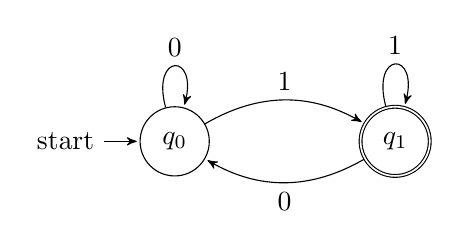
\begin{tikzpicture}[>=stealth',shorten >=1pt,auto,node distance=2.8cm]
    \node[initial, state]            (q0) {$q_0$};
    \node[state, accepting] (q1) [right of=q0] {$q_1$};

    \path[->]
    (q0) edge [bend left]  node {$1$} (q1)
    (q0) edge [loop above] node {$0$} (q0)
    (q1) edge [bend left]  node {$0$} (q0)
    (q1) edge [loop above] node {$1$} (q1)
    ;
  \end{tikzpicture}
\end{center}


% ============================================================
\section{DFA: Grid Layout}

A DFA with states in a 2x2 grid (e.g., tracking two properties).

\begin{center}
  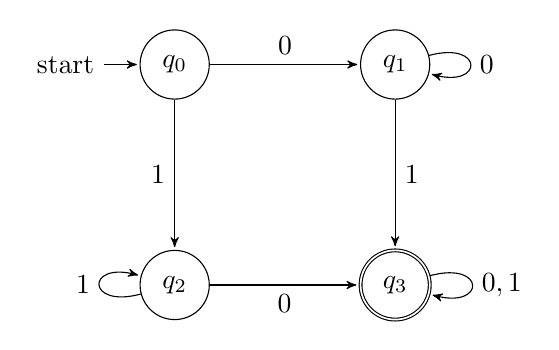
\begin{tikzpicture}[>=stealth',shorten >=1pt,auto,node distance=2.8cm]
    \node[initial, state]   (q0) {$q_0$};
    \node[state]            (q1) [right of=q0] {$q_1$};
    \node[state]            (q2) [below of=q0] {$q_2$};
    \node[state, accepting] (q3) [below of=q1] {$q_3$};

    \path[->]
    (q0) edge              node[above] {$0$} (q1)
    (q0) edge              node[left]  {$1$} (q2)
    (q1) edge              node[right] {$1$} (q3)
    (q1) edge [loop right] node        {$0$} (q1)
    (q2) edge [loop left]  node        {$1$} (q2)
    (q2) edge              node[below] {$0$} (q3)
    (q3) edge [loop right] node        {$0,1$} (q3)
    ;
  \end{tikzpicture}
\end{center}


% ============================================================
\section{DFA: Modular Arithmetic (mod 3)}

Accepts binary strings whose numeric value is divisible by 3.

\begin{center}
  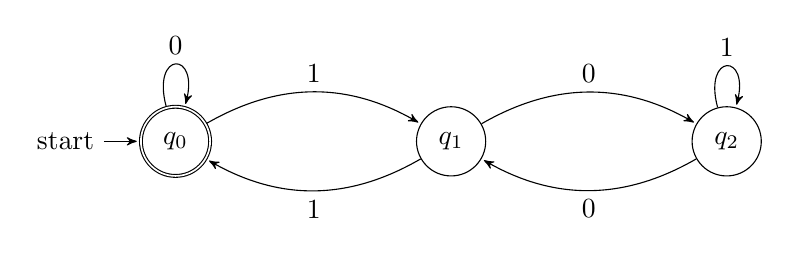
\begin{tikzpicture}[>=stealth',shorten >=1pt,auto,node distance=3.5cm]
    \node[initial, state, accepting] (q0) {$q_0$};
    \node[state]                     (q1) [right of=q0] {$q_1$};
    \node[state]                     (q2) [right of=q1] {$q_2$};

    \path[->]
    (q0) edge [loop above]  node        {$0$} (q0)
    (q0) edge [bend left]   node[above] {$1$} (q1)
    (q1) edge [bend left]   node[below] {$1$} (q0)
    (q1) edge [bend left]   node[above] {$0$} (q2)
    (q2) edge [bend left]   node[below] {$0$} (q1)
    (q2) edge [loop above]  node        {$1$} (q2)
    ;
  \end{tikzpicture}
\end{center}


% ============================================================
\section{NFA: With Epsilon Transitions}

An NFA with $\varepsilon$-transitions.

\begin{center}
  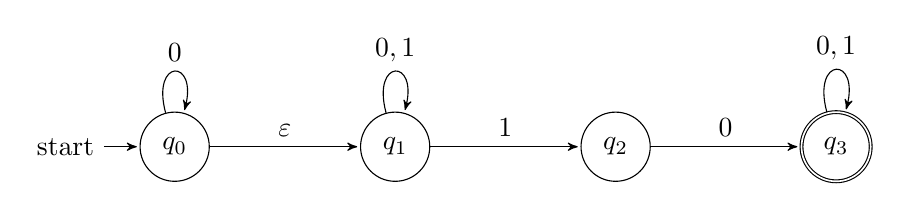
\begin{tikzpicture}[>=stealth',shorten >=1pt,auto,node distance=2.8cm]
    \node[initial, state]   (q0) {$q_0$};
    \node[state]            (q1) [right of=q0] {$q_1$};
    \node[state]            (q2) [right of=q1] {$q_2$};
    \node[state, accepting] (q3) [right of=q2] {$q_3$};

    \path[->]
    (q0) edge              node {$\varepsilon$} (q1)
    (q0) edge [loop above] node {$0$}           (q0)
    (q1) edge              node {$1$}            (q2)
    (q1) edge [loop above] node {$0,1$}         (q1)
    (q2) edge              node {$0$}            (q3)
    (q3) edge [loop above] node {$0,1$}         (q3)
    ;
  \end{tikzpicture}
\end{center}


% ============================================================
\section{NFA: Nondeterministic Branching}

An NFA that accepts strings containing the substring ``01''.

\begin{center}
  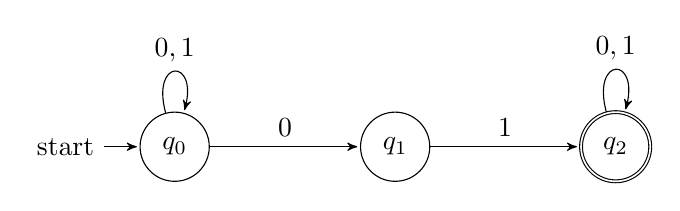
\begin{tikzpicture}[>=stealth',shorten >=1pt,auto,node distance=2.8cm]
    \node[initial, state]   (q0) {$q_0$};
    \node[state]            (q1) [right of=q0] {$q_1$};
    \node[state, accepting] (q2) [right of=q1] {$q_2$};

    \path[->]
    (q0) edge [loop above] node {$0,1$} (q0)
    (q0) edge              node {$0$}   (q1)
    (q1) edge              node {$1$}   (q2)
    (q2) edge [loop above] node {$0,1$} (q2)
    ;
  \end{tikzpicture}
\end{center}


% ============================================================
\section{PDA: Pushdown Automaton}

A PDA for $\{0^n 1^n \mid n \ge 0\}$.

\begin{center}
  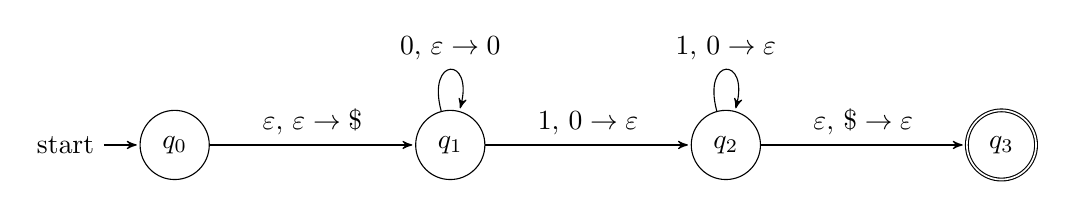
\begin{tikzpicture}[>=stealth',shorten >=1pt,auto,node distance=3.5cm]
    \node[initial, state]   (q0) {$q_0$};
    \node[state]            (q1) [right of=q0] {$q_1$};
    \node[state]            (q2) [right of=q1] {$q_2$};
    \node[state, accepting] (q3) [right of=q2] {$q_3$};

    \path[->]
    (q0) edge              node {$\varepsilon,\, \varepsilon \to \$$}   (q1)
    (q1) edge [loop above] node {$0,\, \varepsilon \to 0$}             (q1)
    (q1) edge              node {$1,\, 0 \to \varepsilon$}             (q2)
    (q2) edge [loop above] node {$1,\, 0 \to \varepsilon$}             (q2)
    (q2) edge              node {$\varepsilon,\, \$ \to \varepsilon$}   (q3)
    ;
  \end{tikzpicture}
\end{center}

PDA transitions use the notation: $\text{input},\, \text{pop} \to \text{push}$.


% ============================================================
\section{Turing Machine}

A TM that accepts $\{0^n 1^n \mid n \ge 1\}$.

\begin{center}
  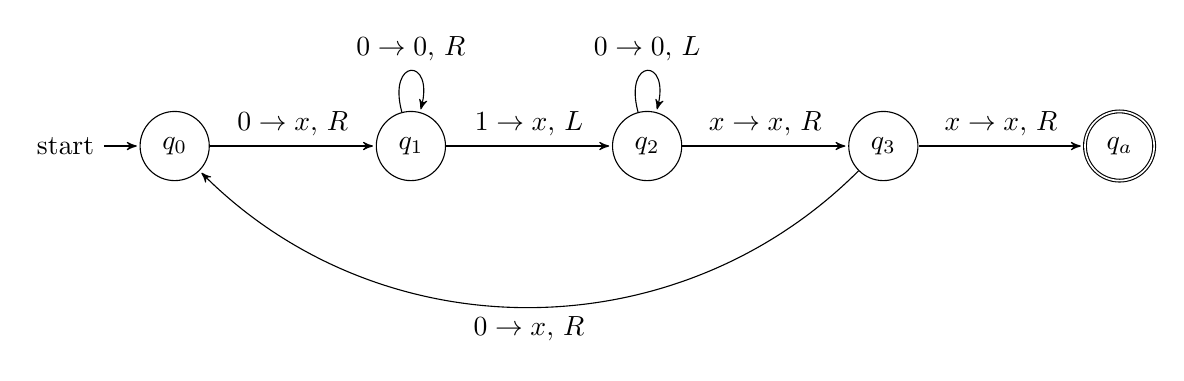
\begin{tikzpicture}[>=stealth',shorten >=1pt,auto,node distance=3cm]
    \node[initial, state]   (q0)                {$q_0$};
    \node[state]            (q1) [right of=q0]  {$q_1$};
    \node[state]            (q2) [right of=q1]  {$q_2$};
    \node[state]            (q3) [right of=q2]  {$q_3$};
    \node[state, accepting] (qa) [right of=q3]  {$q_a$};

    \path[->]
    (q0) edge              node[above] {$0 \to x,\, R$}  (q1)
    (q1) edge [loop above] node        {$0 \to 0,\, R$}  (q1)
    (q1) edge              node[above] {$1 \to x,\, L$}  (q2)
    (q2) edge [loop above] node        {$0 \to 0,\, L$}  (q2)
    (q2) edge              node[above] {$x \to x,\, R$}  (q3)
    (q3) edge [bend left=45] node[below] {$0 \to x,\, R$}  (q0)
    (q3) edge              node[above] {$x \to x,\, R$}  (qa)
    ;
  \end{tikzpicture}
\end{center}

TM transitions use the notation: $\text{read} \to \text{write},\, \text{direction}$.


% ============================================================
%  PART VI: CONTEXT-FREE GRAMMARS
% ============================================================

\section{Context-Free Grammar}

A CFG for $\{0^n 1^n \mid n \ge 0\}$:
\[
  \begin{aligned}
    S &\to 0S1 \mid \varepsilon
  \end{aligned}
\]

A CFG for balanced parentheses:
\[
  \begin{aligned}
    S &\to SS \mid (S) \mid \varepsilon
  \end{aligned}
\]

A more elaborate grammar with multiple productions:
\[
  \begin{aligned}
    S &\to AB \mid \varepsilon \\
    A &\to aAb \mid ab         \\
    B &\to cB \mid c
  \end{aligned}
\]


% ============================================================
\section{Parse Tree}

Using \texttt{tikz-qtree} for parse trees:

\begin{center}
  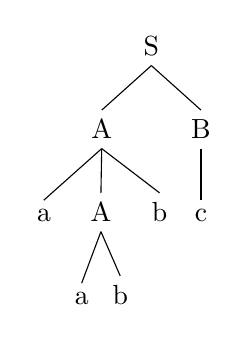
\begin{tikzpicture}
    \Tree
    [.S
      [.A
        [.a ]
        [.A
          [.a ]
          [.b ]
        ]
        [.b ]
      ]
      [.B
        [.c ]
      ]
    ]
  \end{tikzpicture}
\end{center}


% ============================================================
\section{Derivation Steps}

A leftmost derivation:
\[
  \begin{aligned}
    S &\Rightarrow AB      && \text{(rule $S \to AB$)}      \\
      &\Rightarrow aAbB    && \text{(rule $A \to aAb$)}     \\
      &\Rightarrow aabbB   && \text{(rule $A \to ab$)}      \\
      &\Rightarrow aabbc   && \text{(rule $B \to c$)}
  \end{aligned}
\]

Using $\Rightarrow^*$ for multi-step derivation:
\[
  S \Rightarrow^* aabbc
\]


% ============================================================
%  PART VII: REGULAR EXPRESSIONS
% ============================================================

\section{Regular Expressions}

Basic notation:
\[
  \begin{aligned}
    \Sigma &= \{0,1\}                                                \\
    L_1    &= 0^* 1 0^*         && \text{(strings with exactly one 1)} \\
    L_2    &= (0 \cup 1)^*      && \text{(all strings over $\Sigma$)}  \\
    L_3    &= \Sigma^* 01 \Sigma^* && \text{(contains substring 01)}
  \end{aligned}
\]

Common patterns:
\[
  \begin{aligned}
    &\text{At least one $a$:}         & a\Sigma^*  &\cup \Sigma^* a        \\
    &\text{Even length:}              & (\Sigma\Sigma)^*                    \\
    &\text{Starts and ends same:}     & 0\Sigma^* 0 &\cup 1\Sigma^* 1 \cup 0 \cup 1 \cup \varepsilon
  \end{aligned}
\]


% ============================================================
%  PART VIII: COMPLEXITY
% ============================================================

\section{Complexity Classes}

Big-O and related notation:
\[
  f(n) = O(g(n)), \quad f(n) = \Omega(g(n)), \quad f(n) = \Theta(g(n))
\]

Class definitions:
\[
  \begin{aligned}
    \textbf{P}   &= \bigcup_{k \ge 0} \text{TIME}(n^k) \\
    \textbf{NP}  &= \bigcup_{k \ge 0} \text{NTIME}(n^k)
  \end{aligned}
\]


% ============================================================
\section{Reduction Notation}

Mapping reduction:
\[
  A \le_m B
\]

If $A \le_m B$ and $B$ is decidable, then $A$ is decidable.

If $A \le_m B$ and $A$ is undecidable, then $B$ is undecidable.


% ============================================================
%  PART IX: COMMON CONSTRUCTIONS
% ============================================================

\section{Labeled Equation References}

Define and reference equations:
\begin{equation}
  \forall a, b \in A,\; f(a) = f(b) \implies a = b \label{eq:sample-ref}
\end{equation}
As shown in \eqref{eq:sample-ref}, the function is injective.


% ============================================================
\section{Enumerate with Custom Labels}

Roman numerals:
\begin{enumerate}[(i)]
  \item First condition
  \item Second condition
  \item Third condition
\end{enumerate}

Alphabetical:
\begin{enumerate}[(a)]
  \item Case $a$
  \item Case $b$
\end{enumerate}


% ============================================================
\section{Verbatim / Pseudocode}

\begin{verbatim}
DECIDE(w):
  Simulate M on w for |w|^2 steps
  If M accepts, ACCEPT
  If M rejects or loops, REJECT
\end{verbatim}


% ============================================================
\section{Including External Files}

Include a full PDF:
\begin{verbatim}
\includepdf[pages=-,pagecommand={},width=\textwidth]{solution.pdf}
\end{verbatim}

Include an image:
\begin{verbatim}
\begin{center}
  \includegraphics[width=0.8\linewidth]{screenshot.png}
\end{center}
\end{verbatim}


% ============================================================
\section{Spacing Reference}

\begin{center}
  \begin{tabular}{ll}
    \verb|\quad|    & medium space (1em)   \\
    \verb|\qquad|   & large space (2em)    \\
    \verb|\,|       & thin space           \\
    \verb|\;|       & medium-thin space    \\
    \verb|\medskip| & vertical medium skip \\
    \verb|\bigskip| & vertical big skip    \\
    \verb|\pagebreak| & force new page     \\
  \end{tabular}
\end{center}


% ============================================================
\section{Useful Symbols Quick Reference}

\begin{center}
  \begin{tabular}{lll}
    Symbol & Command & Usage \\
    \hline
    $\varepsilon$   & \verb|\varepsilon|   & empty string           \\
    $\emptyset$     & \verb|\emptyset|     & empty set              \\
    $\Sigma$        & \verb|\Sigma|        & alphabet               \\
    $\delta$        & \verb|\delta|        & transition function    \\
    $\vdash$        & \verb|\vdash|        & yields / proves        \\
    $\therefore$    & \verb|\therefore|    & therefore              \\
    $\implies$      & \verb|\implies|      & implies (long arrow)   \\
    $\iff$          & \verb|\iff|          & if and only if         \\
    $\le_m$         & \verb|\le_m|         & mapping reducible      \\
    $\Rightarrow$   & \verb|\Rightarrow|   & derives (grammar)      \\
    $\langle M \rangle$ & \verb|\langle M \rangle| & encoding of $M$ \\
    $\overline{L}$  & \verb|\overline{L}|  & complement             \\
    $\mathcal{P}$   & \verb|\mathcal{P}|   & power set              \\
    $\mathbb{N}$    & \verb|\mathbb{N}|    & natural numbers        \\
    $\infty$        & \verb|\infty|        & infinity               \\
  \end{tabular}
\end{center}

\end{document}